\documentclass{article}
%
%
%	LaTeX template
%
%	vector_spaces_quantum_mechanics.tex
%
%	David Meyer
%	dmm613@gmail.com
%	13 Mar 2024
%
%
%   get various packages
%
\usepackage[margin=1.00in]{geometry}                                    % adjust margins
\geometry{letterpaper}                                                  % or a4paper or a5paper or ... 
\usepackage{url}                                                        % need this to use URLs in bibtex
\usepackage{setspace}                                                   % need this for \setstrech{...}
\usepackage{scrextend}                                                  % need this for addmargin
\usepackage[export]{adjustbox}                                          % need this to get frame for includegraphics
%
%   tikz et al
%
\usepackage{tikz}
\usetikzlibrary{calc,patterns,angles,quotes,shapes,math,decorations,
                through,intersections,lindenmayersystems,backgrounds,
                hobby}
\tikzset{>=latex}                                                       % default to LaTeX arrow head
\usepackage{circuitikz}                                                 % draw circuits    
\usepackage{pgfplots}
%
%	more math stuff
%
\usepackage{amsmath,amsfonts,amssymb,amsthm}
\usepackage{bm}
\usepackage{mathtools}
\usepackage{commath}                                                    % get \norm{x}
\usepackage{fixmath}                                                    % get \mathbold
\usepackage{gensymb}                                                    % get \degree
\usepackage{mathrsfs}
\usepackage{hyperref}
\usepackage{subcaption}
\usepackage{authblk}                                                    % comment out if using beamer (stops \author{} from working in beamer)
\usepackage{graphicx}
\usepackage{hyperref}
\usepackage{alltt}
\usepackage{xcolor}
\usepackage{colortbl}                                                   % \rowcolor{yellow!75} etc
\usepackage{float}
\usepackage{braket}
\usepackage{siunitx}
\usepackage{relsize}
\usepackage{multirow}
\usepackage{esvect}
\usepackage{enumitem}                                                   % use characters instead of numbers in enumerate
\usepackage{changepage}                                                 % needed for \begin{adjustwidth}{-3.25em}{-2.0em} (left justify)
\usepackage{bigints}
\usepackage{multirow}                                                   % \multirow and \multicolumn
%
%	lualatex
%
%	Put this before \documentclass
%
%	!TEX TS-program = LuaLaTeX
%
%
% \usepackage{luatex85,luamplib}
% \usepackage{luacode}
% \mplibnumbersystem{double}
% \mplibtextextlabel{enable}
%
%
%
%	Describe floating point parameters, \fpeval
%
\ExplSyntaxOn
\cs_set_eq:NN \fpeval \fp_eval:n
\ExplSyntaxOff
%
%	Get the x and y components out of a coordinate, e.g.
%
%	\coordinate (EP) at (8,5);
%	\gettikzxy{(EP)}{\slopex}{\slopey}
%
\makeatletter
\newcommand{\gettikzxy}[3]{%
  \tikz@scan@one@point\pgfutil@firstofone#1\relax
  \edef#2{\the\pgf@x}%
  \edef#3{\the\pgf@y}%
}
\makeatother
%
%
%	Watermarks
%
% \usepackage{draftwatermark}
% \SetWatermarkText{Draft}
% \SetWatermarkScale{5}
% \SetWatermarkLightness {0.9} 
% \SetWatermarkColor[rgb]{0.7,0,0}
%
%
%	theorems, definitions, etc
%
\theoremstyle{definition}
\newtheorem{theorem}{Theorem}[section]
\newtheorem{definition}{Definition}[section]
\newtheorem{proposition}{Proposition}[section]
\newtheorem{lemma}{Lemma}[section]
\newtheorem{example}{Example}[section]
\newtheorem{remark}{Remark}[section]
%
%	For drawing matrix products 
%
\newcommand*{\vertbar}{\rule[-1ex]{0.5pt}{2.5ex}}
\newcommand*{\horzbar}{\rule[.5ex]{2.5ex}{0.5pt}}

%
%	The following code allows you to do
%
%	\begin{bmatrix}[r] (or [c] or [l])
%
\makeatletter
\renewcommand*\env@matrix[1][c]{\hskip -\arraycolsep
  \let\@ifnextchar\new@ifnextchar
  \array{*\c@MaxMatrixCols #1}}
\makeatother
%
%	make \arg{min,max}_{n \to \infty} work nicely
%
\newcommand{\argmax}{\operatornamewithlimits{argmax}}
\newcommand{\argmin}{\operatornamewithlimits{argmin}}
%
%	handy commands
%
\newcommand*{\Scale}[2][4]{\scalebox{#1}{$#2$}}
\DeclareMathOperator{\E}{\mathbb{E}}
\DeclareMathOperator{\bda}{\Big \downarrow}						% big down arrow
\newcommand{\veq}{\mathrel{\rotatebox{90}{$=$}}}
%
%	Title, author and date
%
\title{A Bit on Vector Spaces in Quantum Mechanics}
\author{David Meyer \\ \href{mailto:dmm613@gmail.com}
                            {dmm613@gmail.com}}
\date{Last update: \today}
%
%
%
\begin{document}
\maketitle
%
%
%
\section{What is a State in Quantum Mechanics?}
Hilbert space $\mathcal{H}$.
%
%
%
\section{The Real Projective Line}
\label{section:real_projective_line}
The real projective line is the set of all lines that pass
through the origin. One way to think about this is as the
one-dimensional subspace of "rays" 
\cite{youtube:vector_spaces_and_quantum_mechanics,wolfram:ray}. 
This is shown on the left in Figure
\ref{figure:real_projective_line_setup} (or Appendix A).

\bigskip
\noindent
\setstretch{1.25}{If we slide the red point along the $y = 1$
line in Figure \ref{figure:real_projective_line_setup} the angle
$\theta$ varies between $-\frac{\pi}{2}$ and $\frac{\pi}{2}$ as
$x$ varies between $-\infty$ and $\infty$. In particular, as $x
\to \pm\infty$, $\theta \to \pm \frac{\pi}{2}$.  That is \par}

\begin{equation*}
   \lim\limits_{x \to \infty} \theta = \frac{\pi}{2} 
\end{equation*}
\noindent
and
\begin{equation*}
   \lim\limits_{x \to -\infty} \theta = -\frac{\pi}{2} 
\end{equation*}


\vspace{1.00em}

\noindent
If we then look at the points $(x,\theta)$ you find that the real
projective line can be seen as a circle. This is shown on the
right in Figure \ref{figure:real_projective_line_setup}.
%
%
%	A few parameters
%
\setlength			{\fboxsep} {0.50em}						% space between fcolorbox and content
\setlength			{\fboxrule}{0.75pt}						% fcolorbox line thickness
\def \scalefactor	{1.00}									% resizebox scale factor
\def \minipagescale	{0.50}									% minipage scale factor
\def \twidth		{\textwidth}							% point size of points drawn on the cirle
\def \pointsize		{0.50pt}
%
%
%
\vspace{1.75em}
%
%	Draw the picture
%
\begin{figure}[H]
\centering
\fcolorbox{black}{white} {
  \begin{minipage}[t]{\minipagescale \textwidth}
    \centering
    \resizebox{\scalefactor \textwidth}{!}{
      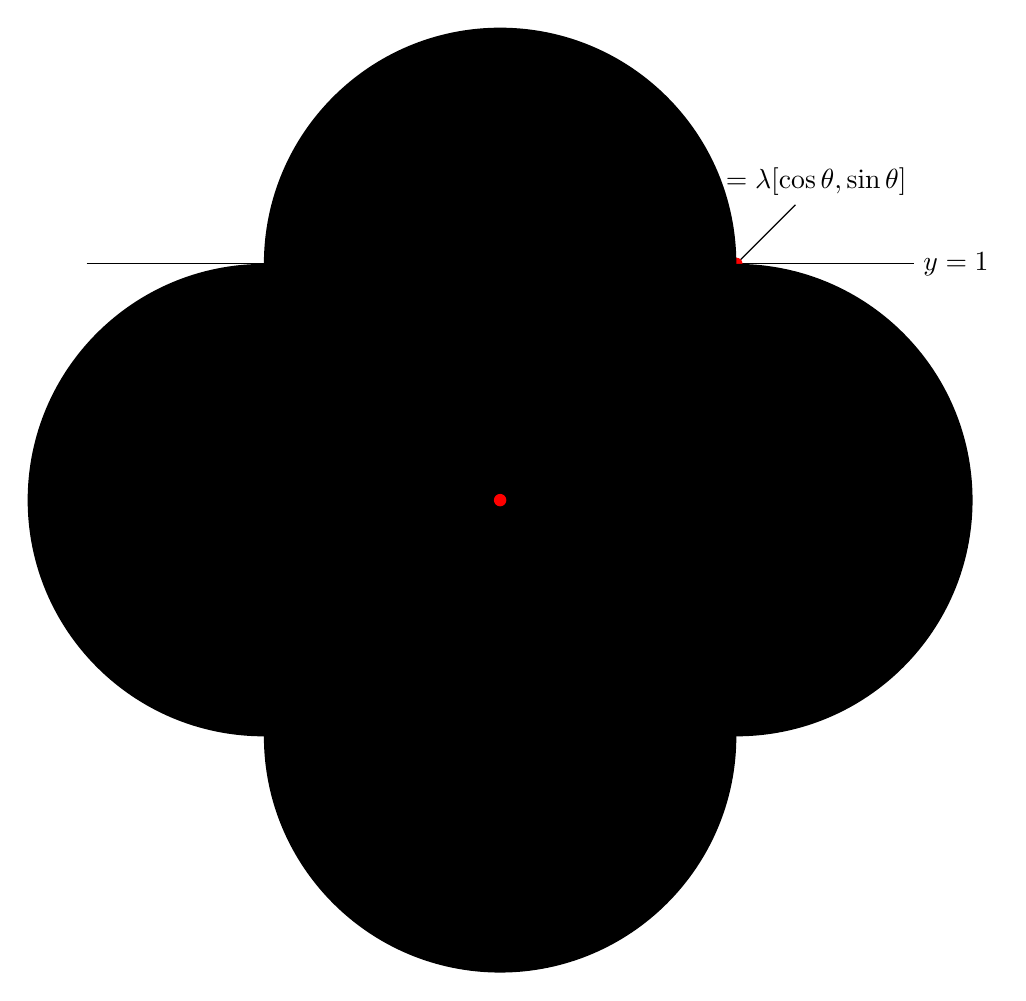
\begin{tikzpicture}[scale=3]
      % Draw the axes
        \draw[-] (-1.75,0) -- (1.75,0) node[below,xshift=-0.15cm]               {$x$};
        \draw[]  (1.50,0)              node[above,xshift=0.25cm]                {$\lambda[1,0]$};
        \draw[-] (0,-0.50) -- (0,1.50) node[right,xshift=0.20cm,yshift=-0.20cm] {$y$};
        \draw[]  (0,1.50)              node[above]                              {$\lambda[0,1]$};
        % Draw the y = 1 line
        \draw [-] (-1.75,1) -- (1.75,1);
        % Draw the y = x line
        \draw [-] (-1.00,-1.00) -- (1.25,1.25) node[above,xshift=-0.25cm] 
        		{$\lambda[x,1] = \lambda [\cos \theta, \sin \theta]$};
        % Intersection of y = 1 and y = x
        \fill [red] (1,1) circle (0.75pt);
        \node [below,yshift=-0.1cm,xshift=0.25cm] at (1,1) {$(1,\frac{\pi}{4})$};
                \node [right,xshift=-0.75cm] at (2,1) {$y = 1$};
        % Draw theta
        \draw [<-] (0.3,0.3) arc (45:90:0.42);
        \node[] at (0.10,0.25) {$\theta$};
        % Draw upper half of unit circle in blue
        \draw [blue,thick] (1,0) arc (0:180:1);
        % Draw bottom half of unit circle in dashed black
        \draw [dashed,thick](-1,0) arc (180:360:1);
        % Put some black points on the unit circle
        \fill [black] (1,0)  circle (\pointsize); 
        \fill [black] (-1,0) circle (\pointsize); 
        \fill [black] (0,1)  circle (\pointsize);
        \fill [black] (0,-1) circle (\pointsize);
        % Draw a dot at the origin
        \fill [red] (0,0) circle (0.75pt);
        % Draw a few coordinates of interest
        \draw (1,0)  node[below]                {$(1,0)$};
        \draw (-1,0) node[below]                {$(-1,0)$};
        \draw (0,1)  node[below,yshift=-0.10cm] {$(0,1)$};
        \draw (0,-1) node[below]                {$(0,-1)$};
      \end{tikzpicture}
      }
  \end{minipage}

%
%	Force the figures to be side by side
%
  \hfill
%
%	Scale the second image
%  
\def \scalefactor {0.775}
\def \minipagescale	{0.50}									% minipage scale factor

%
%	Draw the second figure
%
   \begin{minipage}[t]{\minipagescale \textwidth}
     \centering
     \resizebox{\scalefactor \textwidth}{!}{
        
\begin{tikzpicture}[scale=3]
           \draw [blue,thick] (0,0) circle (1); 
           \node[right,xshift=0.20cm] at (1,0) {$(1,\frac{\pi}{4})$};
           \node[above] at (0,1) {$(0,0)$};
           \node[left,xshift=-0.20cm] at (-1,0) {$(-1,-\frac{\pi}{4})$};
           \node[below,yshift=-0.15cm] at (0,-1) {$(-\infty,-\frac{\pi}{2};\infty,\frac{\pi}{2})$};
           \node[] at (1,1) {$\mathbf{(x},\boldsymbol{\theta}\mathbf{)}$};
           \fill [black] (1,0)  circle (\pointsize); 
           \fill [black] (0,1)  circle (\pointsize); 
           \fill [black] (-1,0) circle (\pointsize);
           \fill [black] (0,-1) circle (\pointsize); 
       \end{tikzpicture}
     }
   \end{minipage}
  }
  \caption{Real Projective Line Setup}
  \label{figure:real_projective_line_setup}    
\end{figure}
%
%
%
\vspace{0.5cm}
%
%
%
\section{The Real Projective Plane}
\label{section:the_real_projective_plane}

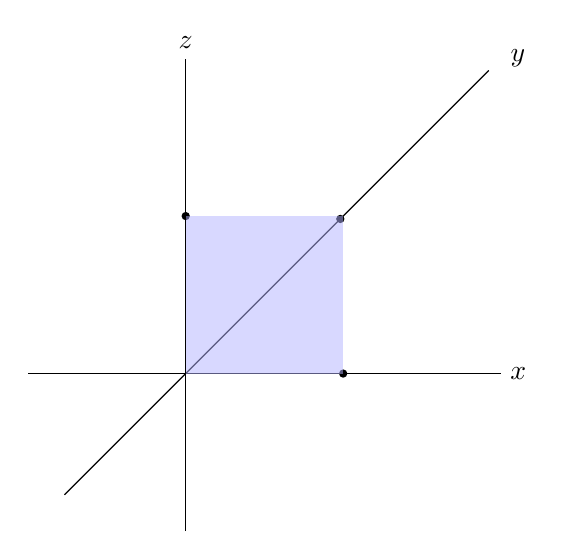
\begin{tikzpicture}[scale=2]
    % Draw axes
    \draw[-] (-1,0,0) -- (2,0,0) node[right] {$x$};
    \draw[-] (0,0,-5) -- (0,0,2) ; % node[below left] {$y$};
    \draw[-] (0,-1,0) -- (0,2,0) node[above] {$z$};
    
    \draw[] (1,1,-2.60) node[right] {$y$};
    
   \fill [black] (0,1,0) circle (0.75pt); % z axis
   \fill [black] (1,0,0) circle (0.75pt); % x axis
   \fill [black] (0,0,-2.55) circle (0.75pt); % y axis

    
    % Draw plane in x-y direction
    \fill[blue!30,opacity=0.5] (0,0,0) -- (1,0,0) -- (1,1,0) -- (0,1,0) -- cycle;
\end{tikzpicture}


%
%
%
\vspace{1.50em}
\section*{Acknowledgements}
\label{section:acknowledgements}
%
%	LaTeX source on overleaf.com
%
\section*{\LaTeX \hspace{0.025 mm} Source}
\url{https://www.overleaf.com/read/gjysgsdftjxy}
%
%	get a bibliography
%
%	Note:.bib files go in ~/Library/texmf/bibtex/bib with TeXShop (MacTeX).
%	You can also use an absolute path, e.g. \bibliography{/Users/dmm/papers/bib/qc}
%
\bibliographystyle{plain}
\bibliography{qc}
%
%
%
\section*{Appendix A: The Real Projective Line}

\setlength			{\fboxsep} {1.00em}						% space between fcolorbox and content
\setlength			{\fboxrule}{0.25pt}						% fcolorbox line thickness
\def \scalefactor	{0.95}									% resizebox scale factor
\def \minipagescale	{0.50}									% minipage scale factor
\def \twidth		{\textwidth}							% resizebox height = \scalefactor * \w

\vspace{0.25cm}
%
%	Draw the picture
%
\begin{figure}[H]
\centering
  \fcolorbox{white}{white} {
    \centering
    \resizebox{\scalefactor \textwidth}{!}{
      \begin{tikzpicture}[scale=3]
      % Draw the axes
        \draw[-] (-1.75,0) -- (1.75,0) node[below,xshift=-0.15cm]               {$x$};
        \draw[]  (1.50,0)              node[above,xshift=0.25cm]                {$\lambda[1,0]$};
        \draw[-] (0,-0.50) -- (0,1.50) node[right,xshift=0.20cm,yshift=-0.20cm] {$y$};
        \draw[]  (0,1.50)              node[above]                              {$\lambda[0,1]$};
        % Draw the y = 1 line
        \draw [-] (-1.75,1) -- (1.75,1);
        % Draw the y = x line
        \draw [-] (-1.00,-1.00) -- (1.25,1.25) node[above,xshift=-0.25cm] 
        		{$\lambda[x,1] = \lambda [\cos \theta, \sin \theta]$};
        % Intersection of y = 1 and y = x
        \fill [red] (1,1) circle (0.75pt);
        \node [below,yshift=-0.1cm,xshift=0.25cm] at (1,1) {$(1,\frac{\pi}{4})$};
                \node [right,xshift=-0.75cm] at (2,1) {$y = 1$};
        % Draw theta
        \draw [<-] (0.3,0.3) arc (45:90:0.42);
        \node[] at (0.10,0.25) {$\theta$};
        % Draw upper half of unit circle in blue
        \draw [blue,thick] (1,0) arc (0:180:1);
        % Draw bottom half of unit circle in dashed black
        \draw [dashed,thick](-1,0) arc (180:360:1);
        % Put some black points on the unit circle
        \fill [black] (1,0)  circle (0.75pt); 
        \fill [black] (-1,0) circle (0.75pt); 
        \fill [black] (0,1)  circle (0.75pt);
        \fill [black] (0,-1) circle (0.75pt);
        % Draw a dot at the origin
        \fill [red] (0,0) circle (0.75pt);
        % Draw a few coordinates of interest
        \draw (1,0)  node[below]                {$(1,0)$};
        \draw (-1,0) node[below]                {$(-1,0)$};
        \draw (0,1)  node[below,yshift=-0.10cm] {$(0,1)$};
        \draw (0,-1) node[below]                {$(0,-1)$};
      \end{tikzpicture}
    }
 }
\end{figure}

%
%	done
%
\end{document} 

